\documentclass{standalone}
\usepackage{times}
\usepackage{mathtools}
\usepackage{amsfonts}
\usepackage{amssymb}

\usepackage{tikz}
\usetikzlibrary{positioning,fit,shapes,calc,decorations.pathreplacing}
\usetikzlibrary{backgrounds}
\usetikzlibrary{arrows.meta}
\usetikzlibrary{shapes,snakes}

\definecolor{processblue}{cmyk}{1,1,1,0}
\definecolor{accent}{rgb}{0.0,0.5,0.8}
\definecolor{accent2}{rgb}{0.8,0.5,0.0}

\begin{document}
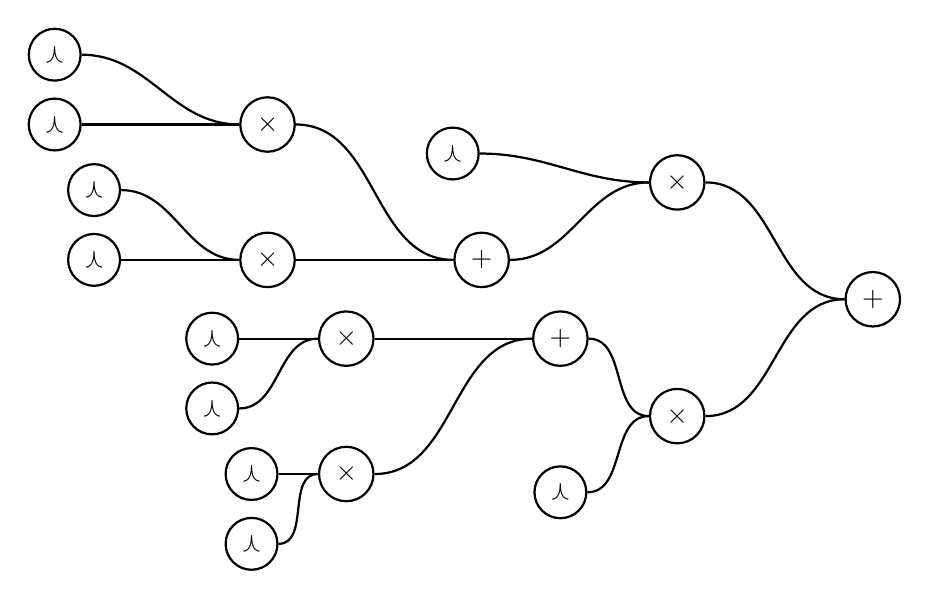
\begin{tikzpicture}[
  node/.style = {
    draw,
    circle,
    thick,
    fill = white,
    minimum width = 0.5cm,
    minimum height = 0.5cm,
  },
  >={Stealth[scale=1.8]},
]

  \node[node] (root) {$+$};

  \node (d1) [left=2cm of root] {};
  \node[node] (p11) [above=of d1] {$\times$};
  \node[node] (p12) [below=of d1] {$\times$};
  \path[-,thick] (p11) edge[out=0,in=180] node {} (root);
  \path[-,thick] (p12) edge[out=0,in=180] node {} (root);

  \node (d21) [left=2cm of p11] {};
  \node[node] (p211) [above left=0cm of d21] {$\curlywedge$};
  \node[node] (p212) [below=0.5cm of d21] {$+$};
  \path[-,thick] (p211) edge[out=0,in=180] node {} (p11);
  \path[-,thick] (p212) edge[out=0,in=180] node {} (p11);

  \node (d22) [left=1.0cm of p12] {};
  \node[node] (p221) [above=0.5cm of d22] {$+$};
  \node[node] (p222) [below=0.5cm of d22] {$\curlywedge$};
  \path[-,thick] (p221) edge[out=0,in=180] node {} (p12);
  \path[-,thick] (p222) edge[out=0,in=180] node {} (p12);

  \node[node] (p312) [left=2cm of p212] {$\times$};
  \node[node] (p311) [above=of p312] {$\times$};
  \path[-,thick] (p311) edge[out=0,in=180] node {} (p212);
  \path[-,thick] (p312) edge[out=0,in=180] node {} (p212);

  \node[node] (p321) [left=2cm of p221] {$\times$};
  \node[node] (p322) [below=of p321] {$\times$};
  \path[-,thick] (p321) edge[out=0,in=180] node {} (p221);
  \path[-,thick] (p322) edge[out=0,in=180] node {} (p221);

  \node[node] (p412) [left=2cm of p311] {$\curlywedge$};
  \node[node] (p411) [above=0.2cm of p412] {$\curlywedge$};
  \path[-,thick] (p411) edge[out=0,in=180] node {} (p311);
  \path[-,thick] (p412) edge[out=0,in=180] node {} (p311);

  \node[node] (p422) [left=1.5cm of p312] {$\curlywedge$};
  \node[node] (p421) [above=0.2cm of p422] {$\curlywedge$};
  \path[-,thick] (p421) edge[out=0,in=180] node {} (p312);
  \path[-,thick] (p422) edge[out=0,in=180] node {} (p312);

  \node[node] (p431) [left=1.0cm of p321] {$\curlywedge$};
  \node[node] (p432) [below=0.2cm of p431] {$\curlywedge$};
  \path[-,thick] (p431) edge[out=0,in=180] node {} (p321);
  \path[-,thick] (p432) edge[out=0,in=180] node {} (p321);

  \node[node] (p441) [left=0.5cm of p322] {$\curlywedge$};
  \node[node] (p442) [below=0.2cm of p441] {$\curlywedge$};
  \path[-,thick] (p441) edge[out=0,in=180] node {} (p322);
  \path[-,thick] (p442) edge[out=0,in=180] node {} (p322);
\end{tikzpicture}
\end{document}
